%% ****** Start of file aiptemplate.tex ****** %
%%
%%   This file is part of the files in the distribution of AIP substyles for REVTeX4.
%%   Version 4.1 of 9 October 2009.
%%
%
% This is a template for producing documents for use with 
% the REVTEX 4.1 document class and the AIP substyles.
% 
% Copy this file to another name and then work on that file.
% That way, you always have this original template file to use.

%\documentclass[aip,graphicx]{revtex4-1}
%\documentclass[aip,reprint]{revtex4-1}

%\usepackage{graphicx}

%\draft % marks overfull lines with a black rule on the right
%\documentclass[pre,aps,floatfix,authordate1-4,twocolumn]{revtex4-1}
%\documentclass[pre,aps,floatfix,authordate1-4]{revtex4-1}

\documentclass[aps,prl,superscriptaddress,twocolumn]{revtex4}



%\documentclass[aps,prl,preprint,groupedaddress]{revtex4}

\usepackage{rotating} 
\usepackage{times}
\usepackage{graphicx}
\usepackage{setspace}
\usepackage{amsmath}
\usepackage{epstopdf}
\usepackage[obeyFinal]{easy-todo}
\usepackage{csquotes}
\usepackage{xr}
\externaldocument{manuscriptPSsuppl}

\begin{document}

% Use the \preprint command to place your local institutional report number 
% on the title page in preprint mode.
% Multiple \preprint commands are allowed.
%\preprint{}

\title{Headgroup structure and cation binding in phosphatidylserine lipid bilayers} %Title of paper

% repeat the \author .. \affiliation  etc. as needed
% \email, \thanks, \homepage, \altaffiliation all apply to the current author.
% Explanatory text should go in the []'s, 
% actual e-mail address or url should go in the {}'s for \email and \homepage.
% Please use the appropriate macro for the type of information

% \affiliation command applies to all authors since the last \affiliation command. 
% The \affiliation command should follow the other information.

\author{Hanne Antila}
\affiliation{Department of Theory and Bio-Systems, Max Planck Institute of Colloids and Interfaces, 14424 Potsdam, Germany}
\author{Pavel Buslaev}
\affiliation{Moscow Institute of Physics and Technology}
\author{Fernando Favela}
\affiliation{Mexico}
\author{Tiago M. Ferreira}
\affiliation{NMR group - Institut for Physics, Martin-Luther University Halle-Wittenberg}
\author{Ivan Gushchin}
\affiliation{Moscow Institute of Physics and Technology}
\author{Matti Javanainen}
\affiliation{Institute of Organic Chemistry and Biochemistry of the 
Czech Academy of Sciences, Flemingovo n\'{a}m. 542/2, CZ-16610 Prague 6, Czech Republic}
\author{Batuhan Kav}
\affiliation{Department of Theory and Bio-Systems, Max Planck Institute of Colloids and Interfaces, 14424 Potsdam, Germany}
\author{Jesper J. Madsen}
\affiliation{Department of Chemistry, The University of Chicago, Chicago, Illinois 60637, United States of America}
\author{Josef Melcr}
\affiliation{Institute of Organic Chemistry and Biochemistry,
Academy of Sciences of the Czech Republic, 
Prague 6, Czech Republic}
\author{Markus Miettinen}
\affiliation{Department of Theory and Bio-Systems, Max Planck Institute of Colloids and Interfaces, 14424 Potsdam, Germany}
\author{Ricky Nencini}
\affiliation{Institute of Organic Chemistry and Biochemistry,
Academy of Sciences of the Czech Republic, 
Prague 6, Czech Republic}
\author{O. H. Samuli Ollila}
\email[]{samuli.ollila@helsinki.fi}
%\homepage[]{Your web page}
\affiliation{Institute of Organic Chemistry and Biochemistry,
Academy of Sciences of the Czech Republic, 
Prague 6, Czech Republic}
\affiliation{Institute of Biotechnology, University of Helsinki}
\author{Thomas Piggot}
\affiliation{Southampton, United Kingdom}
%\author{NMRlipids collaboration}
%\affiliation{nmrlipids.blogspot.fi} 


% Collaboration name, if desired (requires use of superscriptaddress option in \documentclass). 
% \noaffiliation is required (may also be used with the \author command).
%\collaboration{}
%\noaffiliation

\date{\today}

\begin{abstract}
  % insert abstract here
Phosphatidylserine (PS) is a negatively
charged lipid commonly found in eukaryotic membranes, where it interacts with proteins via
electrostatic interactions and direct binding, and can induce
membrane fusion and phase separation in the presence of calcium ions.
Molecular details of these phenomena are not well understood,
because accurate models to interpret the experimental data have not
been available. Here, we use solid-state NMR S-DROSS to measure the signs of the experimental POPS headgroup
order parameters, and gather a set of experimental NMR results from pure PS and mixed PC:PS lipid bilayers. Using the open collaboration
method, we then extract data from a wide range of available PS MD models (force fields) and asses the PS headgroup structures and the ion binding produced by these force fields by comparing to the NMR data. We find that none of the models reproduce the NMR data within experimental accuracy,
but the best ones suggest that the carboxyl group in the serine headgroup
does not rotate freely. In line with the previous results for PC lipids,
none of the PS force fields correctly captures the cation binding affinity---the response of PS headgroups to bound ions can even
\emph{qualitatively} differ from experiments. The collected experimental dataset and simulation
results pave the way for improvement of lipid force fields to correctly
describe the biologically relevant negatively charged membranes and their interactions with ions.
This work is part of the NMRlipids open collaboration project (\url{nmrlipids.blogspot.fi}).
\end{abstract}

%\pacs{}% insert suggested PACS numbers in braces on next line

\maketitle %\maketitle must follow title, authors, abstract and \pacs

% Body of paper goes here. Use proper sectioning commands. 
% References should be done using the \cite, \ref, and \label commands


%\label{}
\section{Introduction}
Phosphatidylserine (PS) is the most common negatively
charged lipid in eukaryotic membranes. In red blood cells, for example,
PS lipids compose 8.5\% of the total lipid weight. 
The abundance, however, varies between different organelles, and up to
25-35\% of the cytosolic leaflet of plasma membranes \cite{lemmon08,leventis10,li14} consists of PS lipids.
PS lipids are vastly important biomolecules that interact with
signaling proteins \cite{leventis10}, regulate
surface charge and protein localization \cite{yeung08}, and
induce protein aggregation \cite{zhao04,gorbenko06}.
Some protein domains interact specifically with PS lipids,
while other protein sites attract PS lipids by nonspecific electrostatics and the
binding can be regulated by calcium \cite{leventis10}.
Therefore, the deciphering structural details
of lipid headgroups and the details of cation binding
are crucial for understanding the PS-mediated processes in the cell membranes.

Experimental studies have indicated that the
PS headgroup is more rigid than the phosphatidylcholine (PC)
owing to electrostatic interactions or the formation of hydrogen bonding network between the headgroups~\cite{browning80,buldt81}.
While most monovalent ions interact weakly with
PS-containing bilayers, multivalent cations and Li$^+$ are able to form strong
dehydrated molecular complexes with PS lipids \cite{hauser77,kurland79,eisenberg79,hauser83,dluhy83,hauser85,feigenson86,mattai89,roux90,roux91,boettcher11}.
The dehydrated complexes of PS headgroup with calcium ions can even lead to
phase separation \cite{hauser77,kurland79,hauser85,feigenson86,mattai89,roux90,roux91}. Mixing PS lipids with PC lipids reduces their propensity to form strong complexes with multivalent ions and makes the PS headgroup less rigid~\cite{browning80,buldt81,roux90,roux91}.
That said, some studies suggest Ca$^{2+}$ has similar specific binding affinity 
to negatively charged and zwiterionic phospholipids, and that
the increased cation binding to negatively charged lipid bilayers arises only due
to the increased local cation concentration in the membrane vicinity~\cite{seelig90,sinn06}. 


\begin{table*}[htb]
%\begin{sidewaystable*}[!p]
\centering
\caption{The list of MD simulations of pure PS bilayers without additional salt along with the references to the force fields used and the MD trajectories.
  Notation 2$\times$[time] indicates that two independent MD runs was conducted. Additional simulation details are given in the supplementary information.
    %   The lipid force fields named as in our previous work~\cite{botan15}. 
}\label{PSsystems}
%begin{minipage}[t]{\textwidth}
\begin{tabular}{lcrrrrrcc}
%\hline
% some footnotes are not visible in typeset-MS (pdf)
lipid/counter-ions  & force field for lipids / ions  & \footnote{Number of lipid molecules with largest mole fraction}N$_{{\rm l}}$  & \footnote{Number of water molecules}N$_{{\rm w}}$  & \footnote{Simulation temperature}T (K)  & \footnote{Total simulation time}t$_{{\rm sim}}$(ns)  & \footnote{Time used for analysis}t$_{{\rm anal}}$ (ns)  & \footnote{Reference for simulation files}files & \tabularnewline
\hline 
POPS/Na$^{+}$  & CHARMM36 \cite{venable13}  & 128  & 4480  & 298  & 2$\times$500  & 2$\times$100  & \cite{charmm36POPS298K}  & \tabularnewline
POPS/K$^{+}$  & CHARMM36 \cite{venable13}  & 128  & 4480  & 298  & 2$\times$500  & 2$\times$100  & \cite{charmm36POPS298Kpotassium}  & \tabularnewline
POPS/Na$^{+}$  & CHARMM36ua \cite{??} \todoi{Correct citation for CHARMMua DOPS}  & 128  & 4480  & 298  & 2$\times$500  & 2$\times$100  & \cite{charmm36uaPOPS298K}  & \tabularnewline
POPS/Na$^{+}$  & MacRog \cite{maciejewski14}  & 128  & 4480  & 298  & 2$\times$500  & 2$\times$100  & \cite{macrogPOPS298Kcorrect}  & \tabularnewline
POPS/K$^{+}$  & MacRog \cite{maciejewski14}  & 128  & 4480  & 298  & 200  & 150  & \cite{macrogPOPS298KwithK}  & \tabularnewline
POPS/Na$^{+}$  & lipid17 \cite{gould18} / JC \cite{joung08}  & 128  & 4480  & 298  & 2$\times$600  & 2$\times$100  & \cite{lipid17POPSjcions}  & \tabularnewline
POPS/Na$^{+}$  & lipid17 \cite{gould18} / ff99 \cite{aqvist90}  & 128  & 4480  & 298  & 2$\times$600  & 2$\times$100  & \cite{lipid17POPSff99ions}  & \tabularnewline
POPS/Na$^{+}$  & Berger \cite{mukhopadhyay04,??}  & 128  & 4480  & 298  & 2$\times$500  & 2$\times$100  & \cite{bergerPOPS298K}  & \tabularnewline
POPS/Na$^{+}$  & GROMOS-CKPM \cite{??} \todoi{Correct citation(s) for CKP.}  & 128  & 4480  & 298  & 2$\times$500  & 2$\times$100  & \cite{ckp1POPS303K}  & \tabularnewline
POPS/Na$^{+}$  & GROMOS-CKP \cite{??} \todoi{Correct citation(s) for CKP.}  & 128  & 4480  & 298  & 2$\times$500  & 2$\times$100  & \cite{ckp2POPS303K}  & \tabularnewline
POPS/Na$^{+}$  & Slipids \cite{jambeck13}  & 128  & 4480  & 298  & 2$\times$500  & 2$\times$100  & \cite{slipidsPOPS298K}  & \tabularnewline
\hline 
DOPS/Na$^{+}$  & CHARMM36 \cite{venable13}  & 128  & 4480  & 303  & 2$\times$500  & 2$\times$100  & \cite{charmm36DOPS303K}  & \tabularnewline
DOPS/Na$^{+}$  & CHARMM36ua \cite{??} \todoi{Correct citation for CHARMMua DOPS}  & 128  & 4480  & 303  & 2$\times$500  & 2$\times$100  & \cite{charmm36uaDOPS303K}  & \tabularnewline
DOPS/Na$^{+}$  & lipid17 \cite{gould18} / JC \cite{joung08}  & 128  & 4480  & 303  & 2$\times$600  & 2$\times$100  & \cite{lipid17DOPSjcions}  & \tabularnewline
DOPS/Na$^{+}$  & lipid17 \cite{gould18} / ff99 \cite{aqvist90}  & 128  & 4480  & 303  & 2$\times$600  & 2$\times$100  & \cite{lipid17DOPSff99ions}  & \tabularnewline
DOPS/Na$^{+}$  & Berger \cite{mukhopadhyay04,??}  & 128  & 4480  & 303  & 2$\times$500  & 2$\times$100  & \cite{bergerDOPS303K}  & \tabularnewline
DOPS/Na$^{+}$  & GROMOS-CKPM \cite{??} \todoi{Correct citation(s) for CKP.}  & 128  & 4480  & 303  & 2$\times$500  & 2$\times$100  & \cite{ckp1DOPS303K}  & \tabularnewline
DOPS/Na$^{+}$  & GROMOS-CKP \cite{??} \todoi{Correct citation(s) for CKP.}  & 128  & 4480  & 303  & 2$\times$500  & 2$\times$100  & \cite{ckp2DOPS303K}  & \tabularnewline
DOPS/Na$^{+}$  & Slipids \cite{jambeck13}  & 128  & 4480  & 303  & 2$\times$500  & 2$\times$100  & \cite{slipidsDOPS303K}  & \tabularnewline
DOPS/Na$^{+}$  & Slipids \cite{jambeck13}  & 288  & 11232  & 303  & 200  & 100  & \cite{slipidsDOPSfiles}  & \tabularnewline
\end{tabular}
%\end{minipage}
%\end{sidewaystable*} 
\end{table*}


The molecular level interpretation of these observations is,
however, lacking, and  classical molecular dynamics (MD) simulations have been widely used in efforts to
to understand the PS headgroup structure, its influence on lipid bilayer properties, and its
interaction with
ions \cite{cascales96,pandit02,mukhopadhyay04,pedersen06,vernier09,boettcher11,molina12,jurkiewicz12,venable13,pan14,vangaveti14,melcrova16,valentine18,hallock18}.
Unfortunately, the results have depended on the force field used.
For example, recent simulations using the NBfix parameters for calcium \cite{kim16} in
CHARMM36 force field \cite{klauda10,venable13}, combined with 2D infrared spectroscopy,
suggest that calcium ions interact only with the carboxylate group of PS lipids \cite{valentine18}; in contrast,
the results from the same lipid model without the NBfix ion parameters, combined with NMR chemical shifts and
rotational-echo double-resonance (REDOR) experiments, indicate a significant binding affinity also to the phosphate region \cite{hallock18}.
Meanwhile, simulations with the Berger force field \cite{berger97,mukhopadhyay04},
combined with fluorescent and vibrational sum frequency spectroscopy, suggest substantial
calcium binding also to the carbonyls in the acyl chains \cite{melcrova16}.

We have recently demonstrated that the lipid C--H bond order parameters, $S_\mathrm{CH}$,
can be utilized to resolve such controversies~\cite{botan15,catte16}. The $S_\mathrm{CH}$ can be
measured from NMR experiments with high accuracy and directly compared to simulations
in order to evaluate the simulation model quality or to interpret the experiments \cite{ollila16}. Using this approach,
it established that the structure of PC lipid headgroup and glycerol backbone are not well
captured by most MD force fields~\cite{botan15}, and that the cation binding to PC
lipid bilayers is overestimated \cite{catte16}.
%
%Based on these data, the cation binding affinity to POPC bilayer has since been improved by implicitly including the electronic polarizability using the electronic continuum correction \cite{melcr18}.
%\todo{Should we leave the mention of ECC out from the Introduction
%(i.e., mention it only in the Conclusions) as the ECC parameters are not used in the paper?} 

Here, we extend the available set of experimentally measured PS lipid headgroup and
glycerol backbone C--H bond order parameters
by measuring the signs of the order parameters using S-DROSS solid-state NMR spectroscopy.
The quality of headgroup structures and the ion binding affinity in
%MD simulations of lipid bilayers containing PS lipids
the available MD simulation models of PS lipids are then asessed based on the collected experimental data.
%using the NMRlipids open collaboration project (\url{nmrlipids.blogspot.fi}).
The results pave the way
for development of lipid models that correctly describe 
the headgroup region of negatively charged lipids in physiological salt
conditions. Such force fields are expected to be useful in understanding
biological function of lipid headgroups and glycerol backbone, as
these are known to behave similarly in simple model membranes and in cells \cite{gally81,scherer87,seelig90}.


\begin{table*}[tb]
%\begin{sidewaystable*}[!p]
\centering
\caption{The list of POPC:POPS mixtures simulated with different molar fractions and different amounts of added calcium. 
  The salt concentrations are calculated as [salt]=N$_{\rm c} \times$[water]\,/\,N$_{\rm w}$, where [water]\,=\,55.5~M.
  This corresponds the concentration in buffer before solvating lipids, which are
  reported in the experiments by Roux et al.~\cite{roux90}.  Notation 2$\times$[time] indicates that two independent MD runs was conducted.
  The simulation details are given in the supplementary information. 
   % The lipid force fields named as in our previous work~\cite{botan15}.
}\label{mixedIONsystems}
%begin{minipage}[t]{\textwidth}
\begin{tabular}{lccccccccc}
lipid/counter-ions  & force field for lipids / ions  & {[}CaCl$_{2}${]}\,(M)  & \footnote{Number of POPC molecules}N$_{{\rm l}}$  & \footnote{Number of water molecules}N$_{{\rm w}}$  & \footnote{Number of additional cations}N$_{{\rm c}}$  & \footnote{Simulation temperature}T (K)  & \footnote{Total simulation time}t$_{{\rm sim}}$(ns)  & \footnote{Time used for analysis}t$_{{\rm anal}}$ (ns)  & \footnote{Reference for simulation files}files\tabularnewline
\hline 
%    POPC:POPS (5:1)/K$^+$  & CHARMM36 \cite{klauda10,venable13} &0  & 110:22 & 4935 & 0  & 298  & 100 & 100 \todoi{Equilibration?} & \cite{charmm36pops+83popcT298K}  \\
POPC:POPS (5:1)/K$^{+}$  & CHARMM36 \cite{klauda10,venable13}  & 0  & 250  & 11207  & 0  & 298  & 200  & 180  & \cite{POPC5POPS1noCaClCHARMM} \tabularnewline
POPC:POPS (5:1)/K$^{+}$  & CHARMM36 \cite{klauda10,venable13}  & 0  & 110  & 4620  & 0  & 298  & 2$\times$500  & 2$\times$100  & \cite{charmm36pops+83popcT298Kpiggot} \tabularnewline
POPC:POPS (5:1)/Na$^{+}$  & CHARMM36 \cite{klauda10,venable13}  & 0  & 110 & 4620  & 0  & 298  & 2$\times$500  & 2$\times$100  & \cite{charmm36pops+83popcT298KpiggotSODIUM} \tabularnewline
POPC:POPS (5:1)  & CHARMM36 \cite{klauda10,venable13,kim16}  & 0.26  & 250 & 11190  & 53  & 298  & 200  & 180  & \cite{POPC5POPS1withCaClCHARMM} \tabularnewline
POPC:POPS (5:1)  & CHARMM36 \cite{klauda10,venable13,kim16}  & 1.06  & 250 & 11174  & 214  & 298  & 200  & 180  & \cite{POPC5POPS1with1MCaClCHARMM} \tabularnewline
POPC:POPS (1:1)/K$^{+}$  & CHARMM36 \cite{klauda10,venable13}  & 0  & 150  & 10785  & 0  & 298  & 200  & 180  & \cite{POPC1POPS1noCaClCHARMM} \tabularnewline
\hline 
POPC:POPS (1:0)  & MacRog \cite{maciejewski14}  & 0  & 120 & 5120  & 0  & 298  & 200  & 150  & \cite{macrogPOPC298K} \tabularnewline
POPC:POPS (5:1)/K$^{+}$  & MacRog \cite{maciejewski14}  & 0  & 120 & 5760  & 0  & 298  & 400 & 250 &  \cite{POPCpopsMACROG}\tabularnewline
POPC:POPS (5:1)/K$^{+}$  & MacRog \cite{maciejewski14}  & 0.10  & 120  & 5760  & 10  & 298  & 600  & 300  & \cite{POPCpopsMACROG} \tabularnewline
POPC:POPS (5:1)/K$^{+}$  & MacRog \cite{maciejewski14}  & 0.30  & 120  & 5760  & 31  & 298  & 600  & 300  & \cite{POPCpopsMACROG} \tabularnewline
POPC:POPS (5:1)/K$^{+}$  & MacRog \cite{maciejewski14}  & 1.00  & 120 & 5760  & 104  & 298  & 600  & 300  & \cite{POPCpopsMACROG} \tabularnewline
POPC:POPS (5:1)/K$^{+}$  & MacRog \cite{maciejewski14}  & 3.00  & 120 & 5760  & 311  & 298  & 600 & 300 & \cite{POPCpopsMACROG}\tabularnewline
\hline 
%    POPC:OPPS (5:1)/K$^+$  & MacRog \cite{maciejewski14} &4.00    & 0   & 120:24 & 5760 & 415  & 298  & 300 & 200 & \cite{POPCpopsMACROGwithK}  \\
POPC:POPS (5:1)/K$^{+}$  & Lipid14/17 \cite{dickson14,gould18}  & 0  & 120  & 5760  & 0  & 298  & 2$\times$500  & 2$\times$200  & \cite{POPCpopsLIPID17withKCI} \tabularnewline
POPC:POPS (5:1)/Na$^{+}$  & Lipid14/17 \cite{dickson14,gould18}  & 0  & 120 & 5760  & 0  & 298  & 2$\times$500  & 2$\times$200  & \cite{POPCpopsLIPID17withNaCI} \tabularnewline
POPC:POPS (5:1)  & Lipid14/17 \cite{dickson14,gould18}  & 0.50  & 120 & 5760  & 52  & 298  & 2$\times$500  & 2$\times$200  & \cite{POPCpopsLIPID17withCaCl} \tabularnewline
POPC:POPS (5:1)  & Lipid14/17 \cite{dickson14,gould18}  & 1.00  & 120  & 5760  & 104  & 298  & 2$\times$500  & 2$\times$200  & \cite{POPCpopsLIPID17withCaCl} \tabularnewline
POPC:POPS (5:1)  & Lipid14/17 \cite{dickson14,gould18}  & 2.00  & 120  & 5760  & 208  & 298  & 2$\times$500  & 2$\times$200  & \cite{POPCpopsLIPID17withCaCl} \tabularnewline
POPC:POPS (5:1)  & Lipid14/17 \cite{dickson14,gould18}  & 3.00  & 120 & 5760  & 311  & 298  & 2$\times$500  & 2$\times$200  & \cite{POPCpopsLIPID17withCaCl} \tabularnewline
POPC:POPS (5:1)  & Lipid14/17 \cite{dickson14,gould18}  & 4.00  & 120  & 5760  & 415  & 298  & 2$\times$500  & 2$\times$200  & \cite{POPCpopsLIPID17withCaCl} \tabularnewline
POPC:POPS (5:1)/Na$^{+}$  & Lipid14/17 \cite{dickson14,gould18}  & 0  & 60 & 3600  & 0  & 298  & 1000  & 1000  & \cite{lipid17_cacl_series} \tabularnewline
POPC:POPS (5:1)/Na$^{+}$  & Lipid14/17 \cite{dickson14,gould18,smith94,dang06}  & 0.08  & 60  & 3561  & 5  & 298  & 1000  & 1000  & \cite{lipid17_cacl_series} \tabularnewline
POPC:POPS (5:1)/Na$^{+}$  & Lipid14/17 \cite{dickson14,gould18,smith94,dang06}  & 0.13  & 60  & 3561  & 8  & 298  & 1000  & 1000  & \cite{lipid17_cacl_series} \tabularnewline
POPC:POPS (5:1)/Na$^{+}$  & Lipid14/17 \cite{dickson14,gould18,smith94,dang06}  & 0.20  & 60 & 3561  & 13  & 298  & 1000  & 1000  & \cite{lipid17_cacl_series} \tabularnewline
POPC:POPS (5:1)/Na$^{+}$  & Lipid14/17 \cite{dickson14,gould18,smith94,dang06}  & 0.41  & 60 & 3522  & 26  & 298  & 1000  & 1000  & \cite{lipid17_cacl_series} \tabularnewline
POPC:POPS (5:1)/Na$^{+}$  & Lipid14/17 \cite{dickson14,gould18,smith94,dang06}  & 0.62  & 60 & 3483  & 39  & 298  & 1000  & 1000  & \cite{lipid17_cacl_series} \tabularnewline
\hline 
POPC:POPS (4:1)/Na$^{+}$  & Berger \cite{tieleman99,mukhopadhyay04}  & 0  & 102 & 4290  & 0  & 310  & 120  & 80  & \cite{bergerPOPSPOPC4:1mixtureT310K} \tabularnewline
POPC:POPS (4:1)  & Berger \cite{tieleman99,mukhopadhyay04}  & 0.102\footnote{\label{noteBerger}Calculation of concetration complicated by the
usage scaled ions. Concentration taken as reported in the delivered
data.}  & 104  & 4306  & 24  & 310  & 300  & 100  & \cite{POPCpopsBERGERwith102mMCa} \tabularnewline
POPC:POPS (4:1)  & Berger \cite{tieleman99,mukhopadhyay04}  & 0.715\textsuperscript{\ref{noteBerger}}  & 104 & 4306  & 72  & 310  & 300  & 100  & \cite{POPCpopsBERGERwith715mMCa} \tabularnewline
\hline 
POPC:POPS (5:1)/Na$^{+}$  & GROMOS-CKP \cite{??}  & 0  & 110 & ?  & 0  & 298  & 2$\times$500  & 2$\times$100  & \cite{POPCpopsGROMOSCKPwithNa} \tabularnewline
POPC:POPS (5:1)/Na$^{+}$  & GROMOS-CKPM \cite{??}  & 0  & 110 & ?  & 0  & 298  & 2$\times$500  & 2$\times$100  & \cite{POPCpopsGROMOSCKPMwithNa} \tabularnewline
\end{tabular}
%\end{minipage}
%end{sidewaystable*} 

\end{table*}

\section{Methods}

\subsection{Experimental C--H bond order parameters}% from the natural abundance $^{13}$C\,NMR}

The headgroup and glycerol backbone C--H bond order parameter magnitudes of 1-palmitoyl-2-oleoyl-{\it sn}-glycero-3-phospho-L-serine (POPS)
were determined by measuring the chemical-shift resolved dipolar splittings
with a R-type Proton Detected Local Field (R-PDLF) experiment~\cite{dvinskikh04}.
The corresponding order parameter signs were measured with a S-DROSS experiment~\cite{gross97}
using natural abundance $^{13}$C solid state NMR spectroscopy as described previously \cite{ferreira13,ferreira16}.
The experiments were done in a Bruker Avance III 400 spectrometer operating at a $^1$H Larmor frequency of 400.03 MHz.
Magic angle spinning (MAS) of the sample was used at a frequency of 5.15 kHz (R-PDLF experiment) and 5 kHz (S-DROSS experiment).
The following experimental setups were used.

{\emph{C--H bond order parameters from the R-PDLF experiment.}} The parameters are described according to Figures 1c and 2c of the original reference
for the R-PDLF experiment~\cite{dvinskikh04}.  The refocused-INEPT delays were $\tau_1=$\,1.94\,ms and $\tau_2=$\,0.97\,ms.
The used radio frequency pulses had the following nutation frequencies: 46.35 kHz (R18$^7_1$ pulses), 63.45 kHz ($^{13}$C 90$^{\rm{o}}$ and 180$^{\rm{o}}$),
50 kHz (SPINAL64 $^1$H decoupling pulses).
The $t_1$ increment was equal to 10.79 $\mu$s $\times18\times2$, and 32 points in the indirect
dimension were recorded using 1024 scans for each, with a recycle delay of 5\,s and a spectral width of 149.5 ppm.

\emph{Order parameter signs from the S-DROSS experiment.}
The parameters are described according to Figures 1b and 1c of the original reference for the S-DROSS
experiment~\cite{gross97}. The refocused-INEPT delay $\delta_2$ was 1.19 ms. The $\tau_1$ and $\tau_2$ in the S-DROSS recoupling
blocks $R$ were set as $\tau_1=$\,39.4\,$\mu$s and $\tau_2=$\,89.4 $\mu$s. The used radio frequency pulses had the nutation
frequencies: 63.45 kHz ($^{13}$C 90$^{\rm{o}}$ and 180$^{\rm{o}}$), 50 kHz ($^1$H\,SPINAL64 decoupling).
The $t_1$ increment (dipolar recoupling dimension) was 800 $\mu$s, and a total of 8 points along $t_1$ were
measured using 1024 scans for each, with a recycle delay of 5\,s and a spectral width of 149.5 ppm.

\emph{Numerical simulations of S-DROSS curves.}
The numerical simulations of S-DROSS curves were performed using the SIMPSON simulation package \cite{bak00}
by inputing the $^{13}$C--$^1$H
dipolar couplings, either as determined by the R-PDLF experiments, or as calculated from the known $^2$H quadrupolar couplings \cite{browning80}.
The chemical shift anisotropy and homonuclear couplings were neglected, and the SIMPSON input file {\it{rep2000}} was used to simulate a random
distribution of bilayer orientations in the samples studied.

\emph{Sample preparation.}
The sample was prepared simply by mixing POPS powder (1-palmitoyl-2-oleoyl-{\it sn}-glycero-3-phospho-L-serine, purchased from Avanti Polar Lipids
as sodium salt) with water (lipid:water 60:40\,wt-\%) in an Eppendorf tube by mixing and centrifuging the sample approximately 5 to 6 times
until a homogeneous viscous fluid was visually observed. Then 20 mg of the sample was transferred to an NMR insert suitable for 4 mm NMR rotors.  


\subsection{Molecular dynamics simulations}
Molecular dynamics simulation data were collected using
the Open Collaboration method \cite{botan15}, with
the NMR\-lipids Project blog (\url{nmrlipids.blogspot.fi}) and
GitHub repository (\url{github.com/NMRlipids/NMRlipidsIVotherHGs})
as the communication platforms.
The simulated systems are listed in 
Tables \ref{PSsystems} (pure PS bilayers without additional ions) 
and \ref{mixedIONsystems} (mixed PC:PS bilayers at various salt concentrations).
Further simulation details are given in the SI, and
the simulation data are indexed in a
searchable database available at \url{www.nmrlipids.fi},
and in the NMRlipids/MATCH repository (\url{github.com/NMRlipids/MATCH}).

The C--H bond order parameters were calculated directly
from the carbon and hydrogen positions using the definition
\begin{equation}
S_{\rm CH}=\frac{1}{2}\langle 3\cos^2\theta -1 \rangle,
\end{equation}
where $\theta$ is the angle between the C--H bond and the membrane normal
(taken to align with $z$, with bilayer periodicity in the $xy$-plane).
Angular brackets denote average over all sampled configurations.
The order parameters were calculated by first averaging over time separately
for each lipid in the system, and then calculating the average and
the standard error of the mean over the different lipids. The analysis was conducted using a
Python program ({\tt calcOrderParameters.py}, available in Ref. \citenum{MATCHgit}) that utilizes the
MDAnalysis library \cite{agrawal11,gowers16}. 
The ion number density profiles were calculated using the {\tt gmx density} tool
of the Gromacs sofware package \cite{gromacsMANUAL}.

\subsection{Comparison of ion binding to negatively charged lipid bilayers 
between simulations and experiments using the molecular electrometer concept}

The order parameters of the $\alpha$ and $\beta$ carbons in the PC headgroup
decrease proportionally to the amount of positive
charge bound to the bilayer \cite{akutsu81,altenbach84,seelig87},
and can therefore be used to measure the ion binding affinity.
This concept, known as the molecular electrometer, is especially useful for 
comparison between simulations and experiments, as
the headgroup order parameters at varying cation
concentrations can be easily calculated from
simulations~\cite{catte16}. The headgroup order parameters
of negatively charged PS and PG lipids also exhibit systematic, but less
understood dependencies on the bound charge~\cite{borle85,macdonald87,roux86,roux90}.
Therefore, measuring the PC headgroup order parameters from 
mixed (here PS:PC) bilayers~\cite{roux86,roux90,roux91} (see also SI section \ref{electrometerFORmixtures}) provides a more straightforward way of characterizing the ion binding to negatively charged membranes.

Calibrating the PC order parameter response to a known amount of bound charge~\cite{catte16,melcr18} is an important preliminary step for using the molecular electrometer concept.
This can be done using experimental data from mixtures of
monovalent cationic surfactants (dihexadecyldimethylammonium) and POPC~\cite{scherer89,melcr18},
(see SI section \ref{electrometerCALIBRATION}). Additionally, we quantify the response of PC headgroup order parameters
to the negatively charged PS, which also follows the molecular electrometer
concept in experiments~\cite{scherer87} (see SI section \ref{electrometerFORmixtures}).

Studies applying the molecular electrometer concept have utilized two different definitions for salt concentration:
the concentrations are reported either in water before solvating the lipids \cite{akutsu81,roux90,catte16},
or in bulk water after solvating the lipids \cite{altenbach84,melcr18}.
In this work, we use the former definition to be consistent with the reference
experimental data \cite{roux90}. However, the choice of definition has only a marginal effect
to the results in simulations with realistic ion binding affinity
(see SI section \ref{concentrationDEFsection}).

\section{Results and Discussion}

\subsection{Headgroup and glycerol backbone order parameters of POPS from $^{13}$C NMR}

\begin{figure}[!tb]
  \centering
  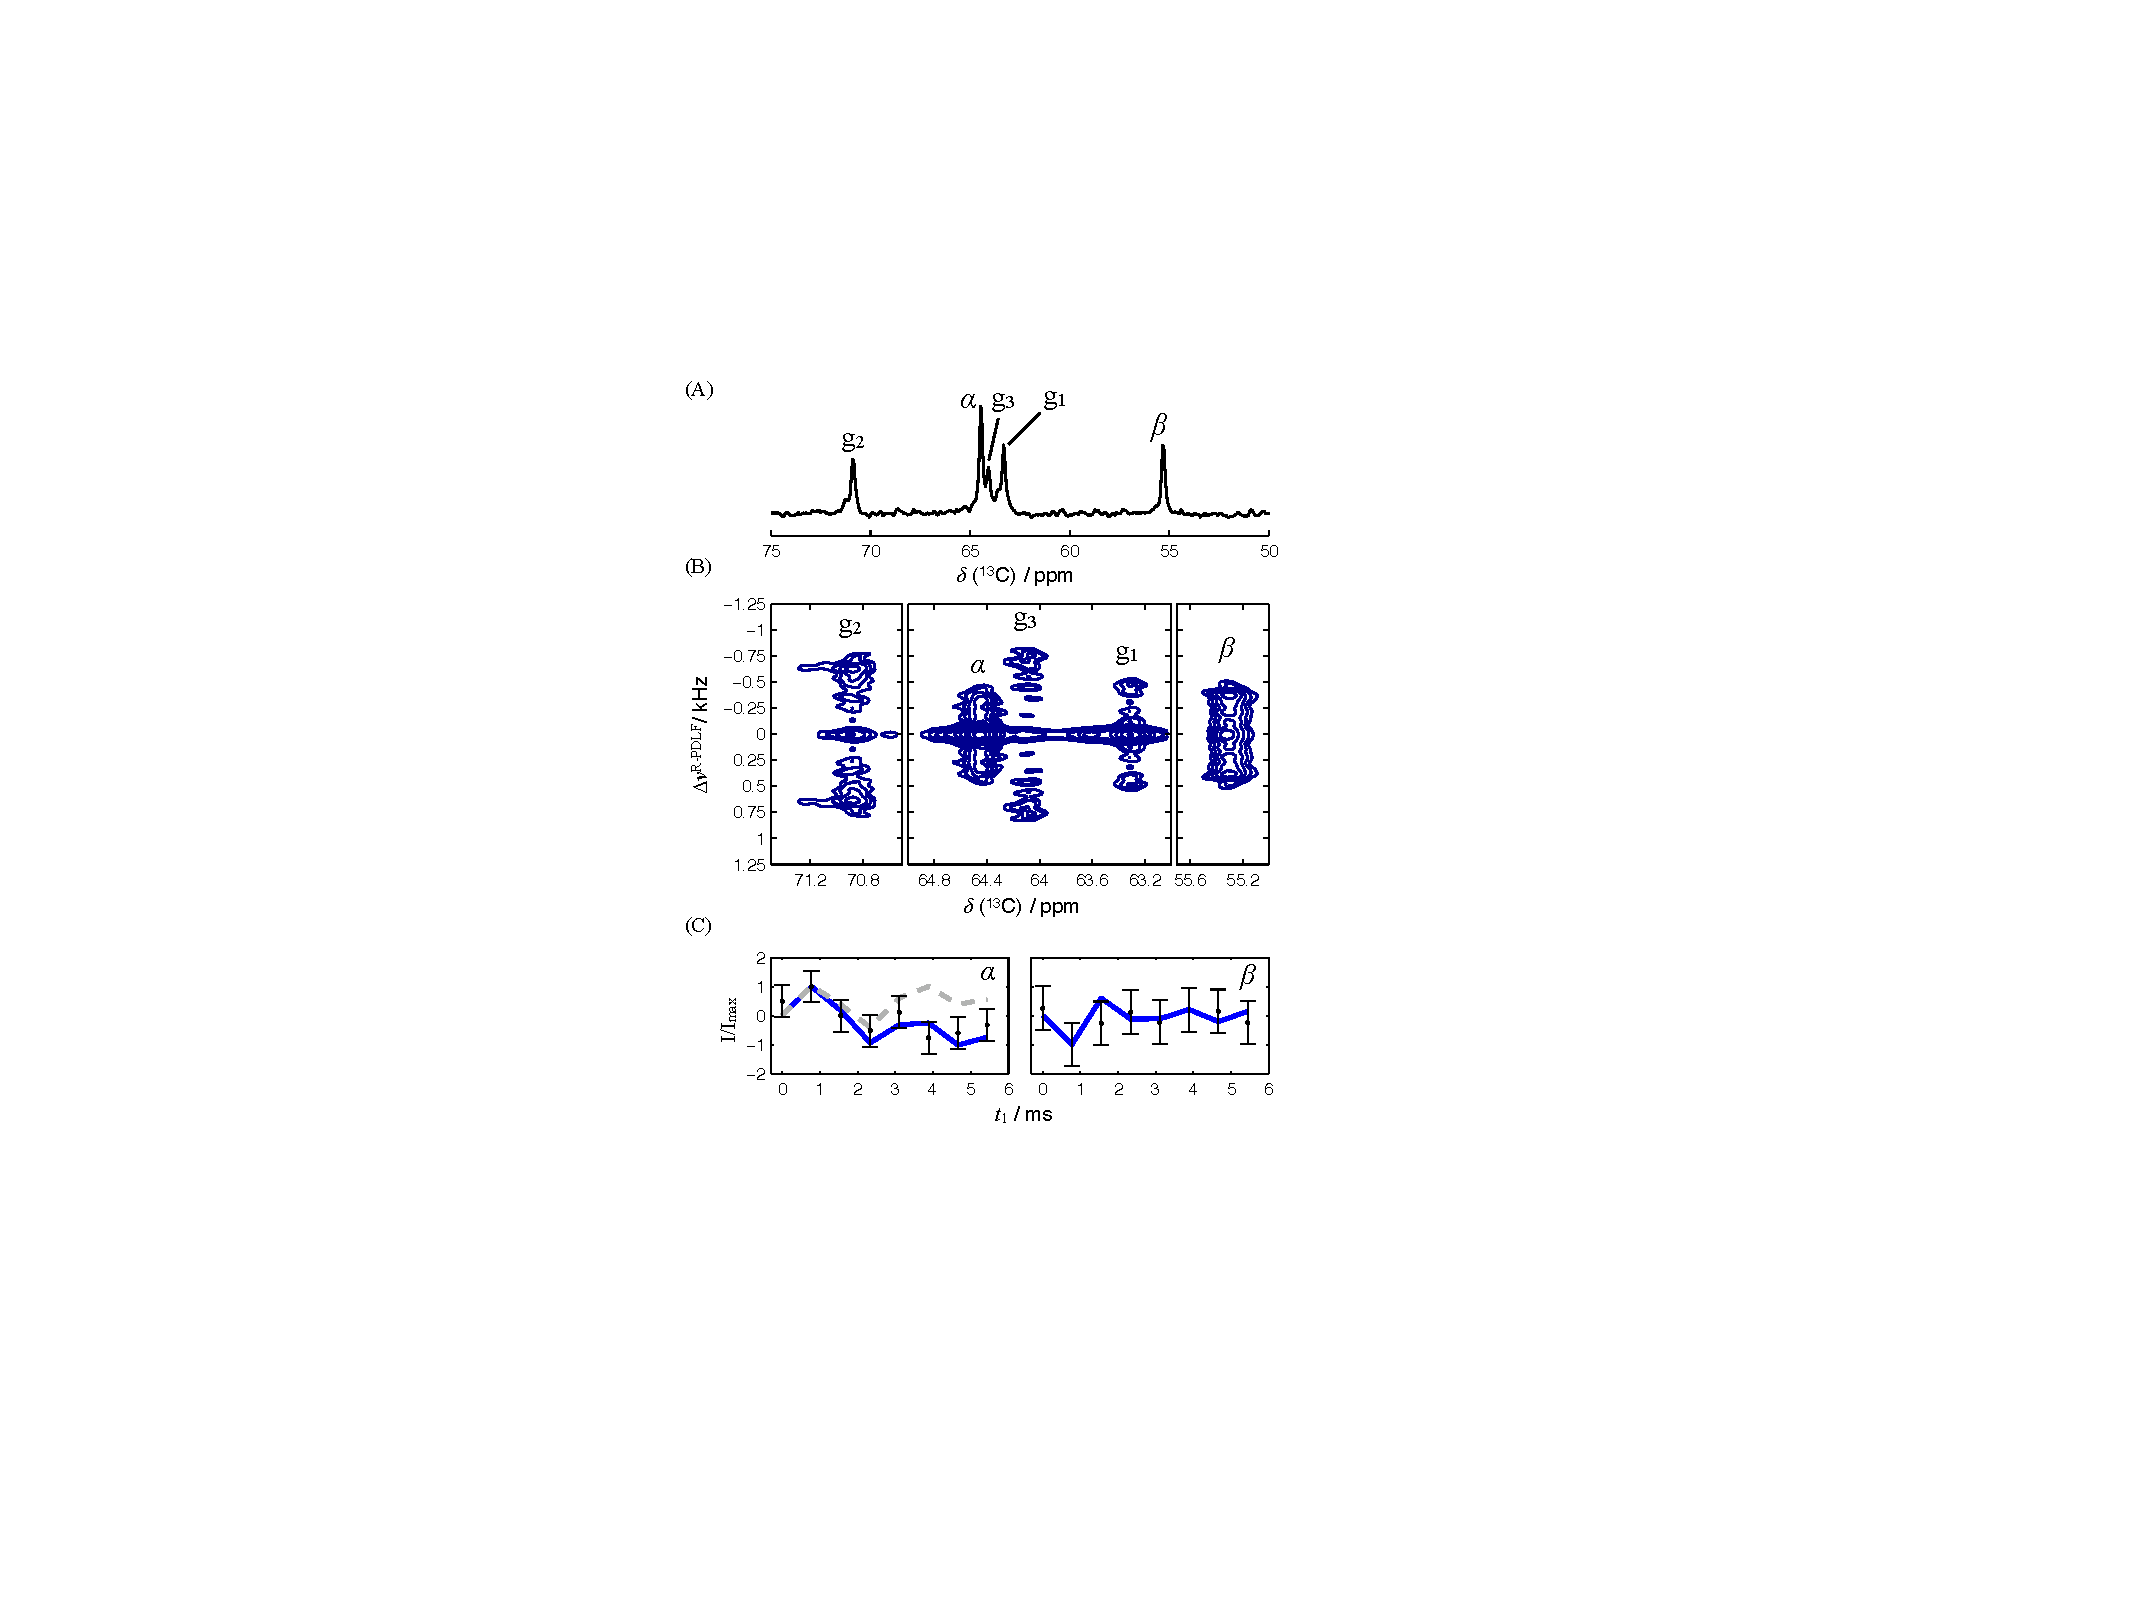
\includegraphics[width=8.5cm]{../Figs/fig1_POPS.pdf}
  \caption{\label{PShgSIGNSsimpson}
    The headgroup and glycerol backbone region of the (A) INEPT spectrum and
    (B) 2D R-PDLF spectra.
    (C) Experimental S-DROSS data (points), and SIMPSON simulations (blue lines) with
    the C--H bond order parameter values of -0.12 for the $\beta$-carbon, and +0.09 and -0.02
    for the $\alpha$-carbon.
    Dashed gray line is the S-DROSS curve from a SIMPSON simulation with a positive value (+0.02) 
    for the smaller $\alpha$-carbon C--H bond order parameter.
  }
\end{figure}
\begin{figure}[!htb]
  \centering
  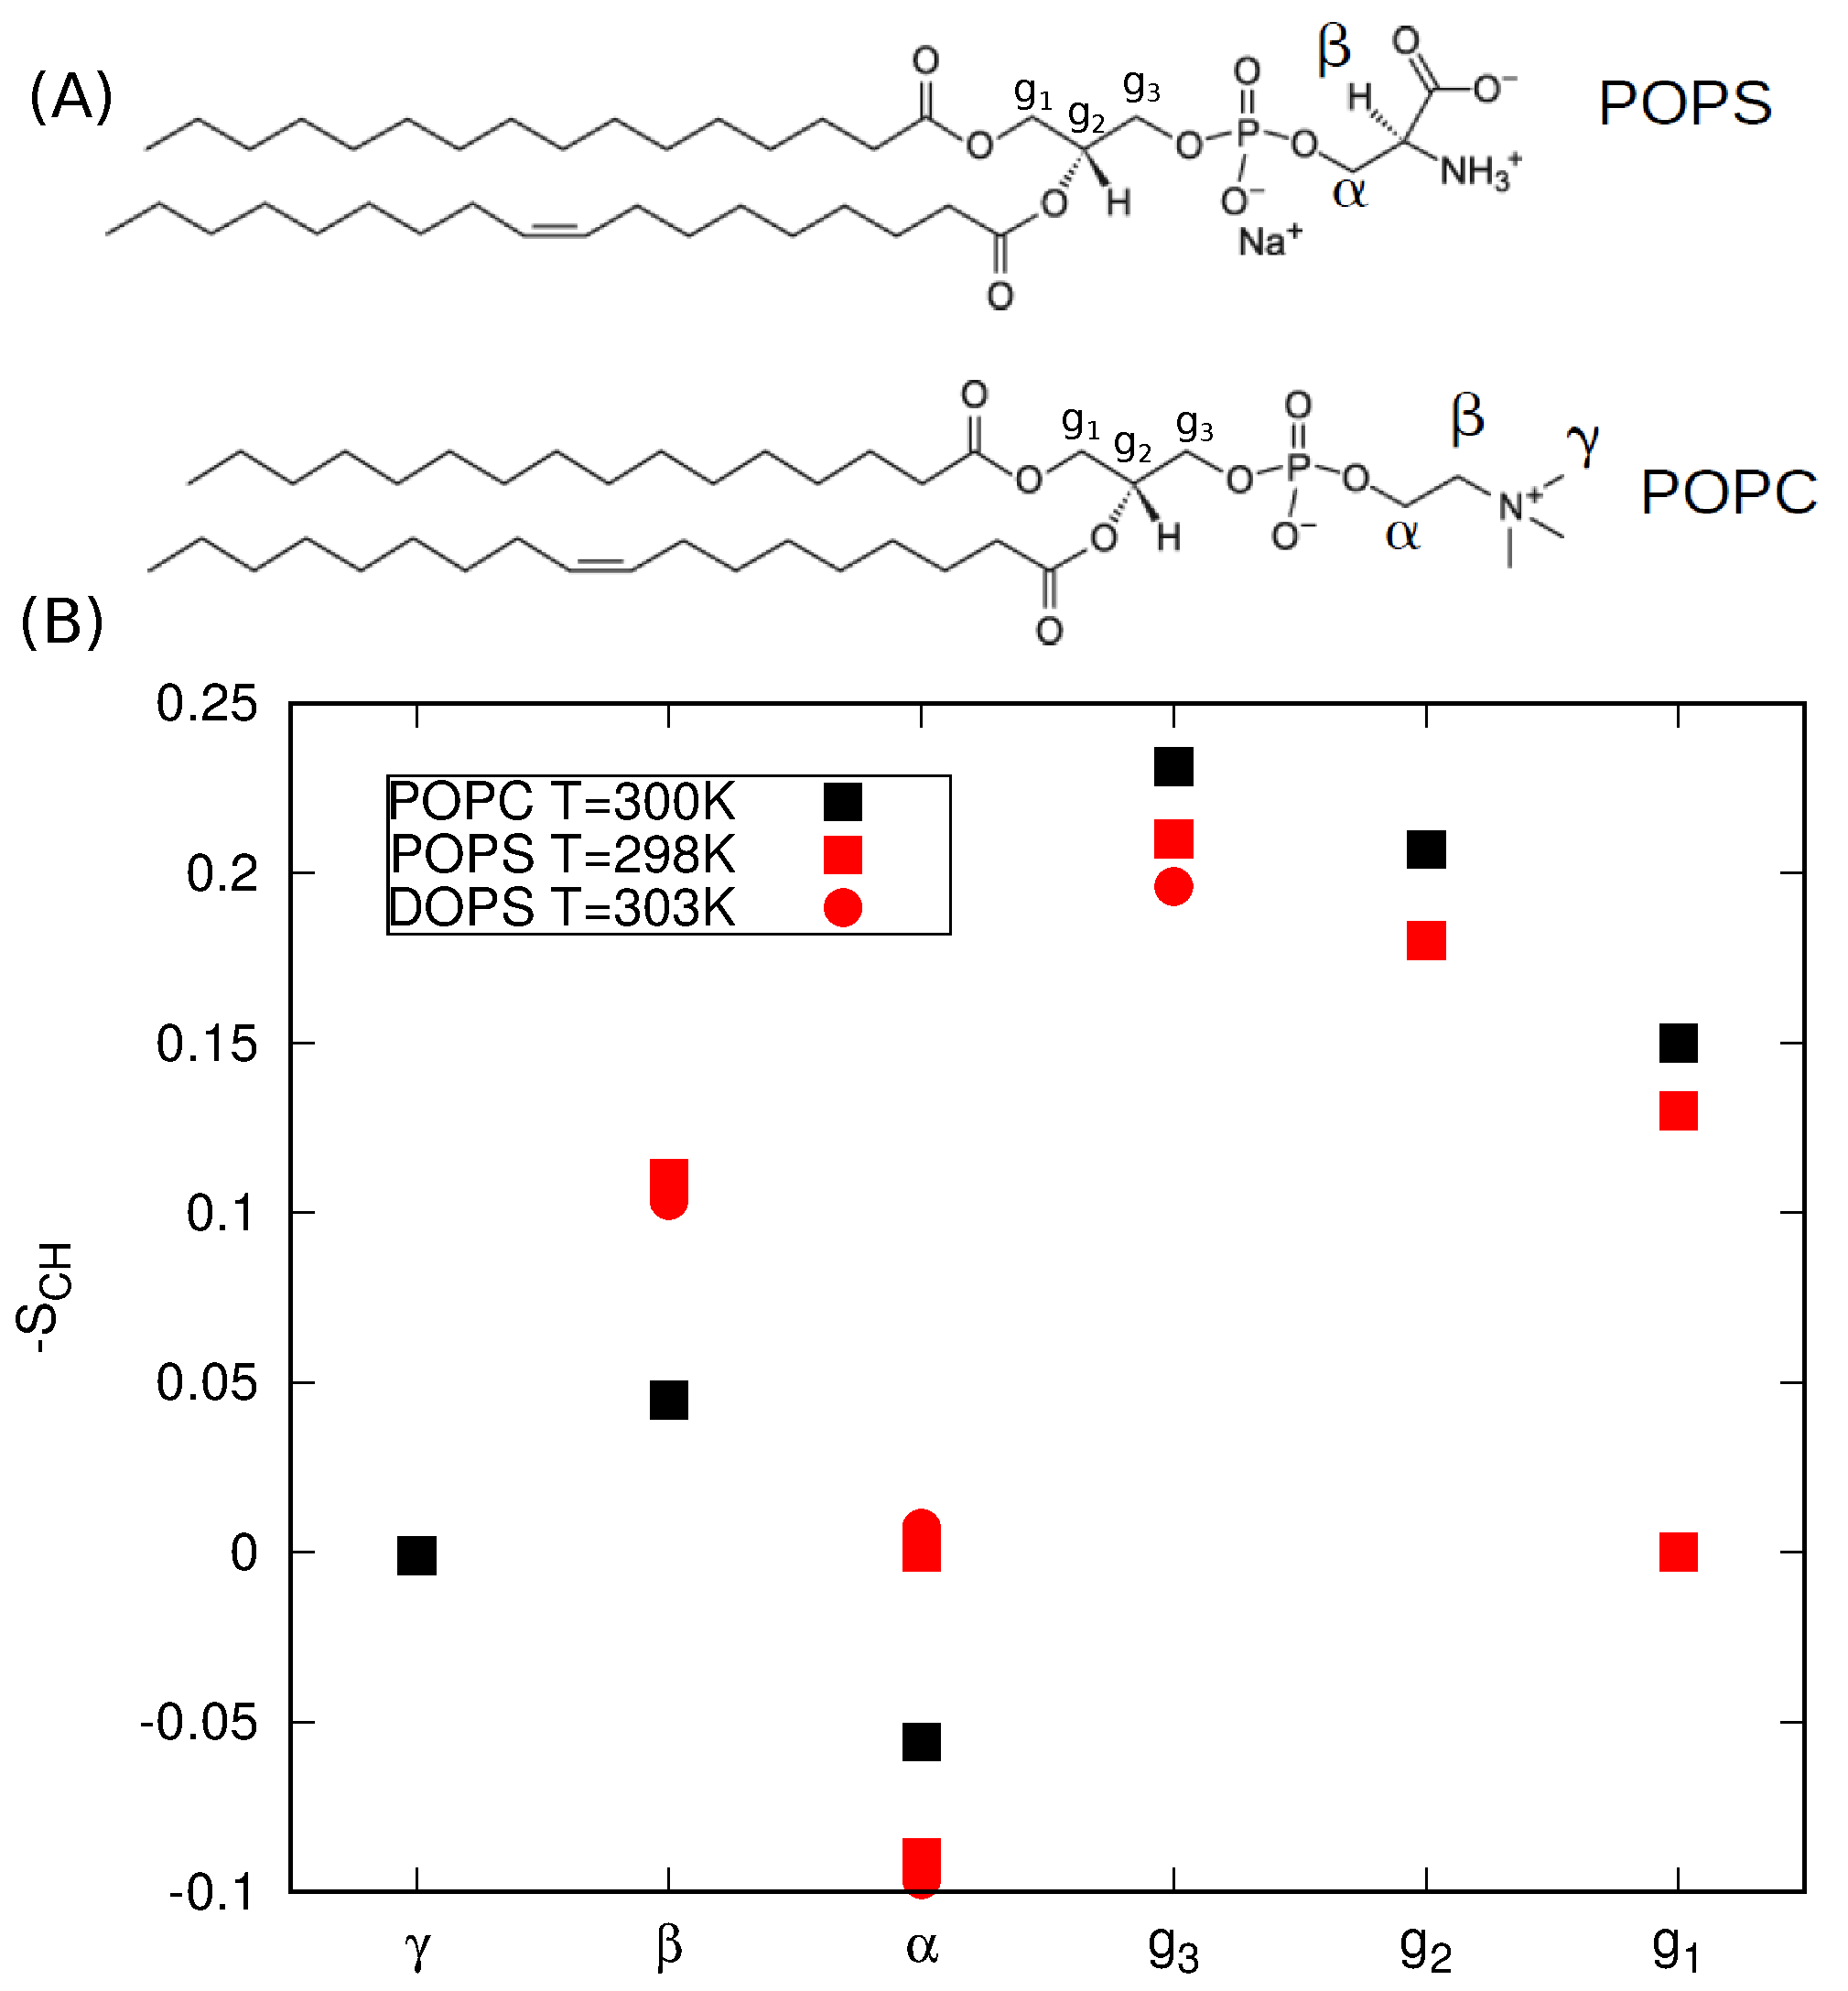
\includegraphics[width=9.0cm]{../Figs/PCPScomp.eps}
  \caption{\label{HGorderParameters}
    (A) Chemical structures and labels for the headgroup and glycerol backbone carbons.
    (B) Headgroup and glycerol backbone order parameters of POPS (T = 298 K) measured in this work compared
    with the previously published values from DOPS (T = 303 K, $^2$H NMR, 0.1M of NaCl) \cite{browning80} and 
    POPC  (T = 300 K, $^{13}$C NMR) \cite{ferreira13} experiments. Signs of the PS order parameters
    are measured in this work whereas signs of the PC order parameters are measured previously~\cite{ferreira16}.
    The size of errorbars ($\pm$0.02) shown for $^{13}$C NMR data is justified previously~\cite{botan15,ollila16}. 
  }
  \todo{Replacing the "literature" with "from Ref X" has been suggested  https://github.com/NMRLipids/NMRlipidsIVotherHGs/issues/34.
  We can do this just before submission when citation numbers will not change anymore.}
\end{figure}

The INEPT and 2D R-PDLF experiments from POPS sample give well resolved spectra for all the
carbons in the headgroup and glycerol backbone regions (Fig. \ref{PShgSIGNSsimpson}).
The glycerol backbone carbon peaks were assigned according to the POPC spectra~\cite{ferreira13} whereas
the peaks for $\beta$ and $\alpha$ carbons were assigned according to the
known order parameters from the $^2$H\,NMR experiments~\cite{browning80}.
Slices of the R-PDLF spectra and the resulting order parameter values
are shown in the supplementary information (Fig. \ref{DPslices}). 

Since the R-PDLF and previous $^2$H\,NMR experiments \cite{browning80,roux91} give 
only the absolute values of order parameters, we determined the signs of the PS headgroup
order parameters using the S-DROSS experiment \cite{gross97}.
For a given carbon, its S-DROSS dipolar modulation profile in the indirect dimension is a superposition
of sinusoidal functions from the possible orientations of crystallites in the sample (or bilayer patches).
We phase corrected the 2D spectrum in the direct dimension such that positive and negative signs for the C—H
bond order parameter give rise to profiles that initially increase and decrease, respectively.
In practice, we use the known negative sign of the acyl chain carbons as a reference to perform
the phase correction and interpret the distinct initial slopes of the S-DROSS profiles (Fig. \ref{DPslices}). 
The S-DROSS slice for the $\beta$-carbon clearly shows an initial decrease and therefore its order parameter must be negative.
For the $\alpha$-carbon such analysis is not as trivial due to the two inequivalent order parameters of the two distinct C—H bonds.
However, the beginning of its S-DROSS slice suggests that the larger order parameter of the alpha-carbon is positive and the
decrease towards negative values at longer $t_1$ suggests that the smaller order parameter is negative.    
%
%The S-DROSS slice clearly shows that the order parameter of
%the $\beta$-carbon is negative (Fig. \ref{PShgSIGNSsimpson} C)), \todo{
%Could we explain in a few words how this is clearly seen?}
%which is confirmed by SIMPSON simulations. The beginning of the S-DROSS slice
%suggests that the larger order parameter of the $\alpha$-carbon 
%is positive and the deviation towards negative values with longer T$_1$ times suggests
%that the smaller order parameter is negative.
%
This is confirmed by a SIMPSON simulation
using the order parameter values of +0.09 from dipolar coupling measured here (Fig. \ref{DPslices})
and -0.02 from the $^2$H\,NMR experiment~\cite{roux91}.
The literature value for the smaller order parameter was used because the
resolution of our R-PDLF experiment was not sufficient to determine the
small value of the order parameter.
The S-DROSS curve from SIMPSON simulation with a positive value for the smaller order parameter
(dashed grey in Fig. \ref{PShgSIGNSsimpson} C)) did not agree with the experiment, 
corroborating the interpretation that the smaller order parameter is negative.

The headgroup and glycerol backbone order parameters of 
POPS measured in this work are in good agreement with the previously reported
values from $^2$H\,NMR experiments of DOPS \cite{browning80} (Fig. \ref{HGorderParameters}).
When compared with the previously measured values for POPC \cite{ferreira13} (Fig. \ref{HGorderParameters}),
the $\beta$-carbon order parameter is significantly more negative and $\alpha$-carbon
experiences substantial forking (different order parameters for the two hydrogens in the same carbon \cite{ollila16}) in the PS headgroup.
These features have been intepreted to arise from a rigid PS headgroup
conformation, stabilized by hydrogen bonds or electrostatic
interactions \cite{browning80,buldt81}, but detailed structrural interpretation is not
available. 
%Moved here from the molecular electrometer paragraph because there it distrupted the flow of the section and it contains results. This also enables referring to figures in order. I also removed the refs which do not seem to refer to the actual data used in the figure.
%Rewrote the paragraph, see if ok.

We note that the the DOPS $^2$H~NMR reference data found in the literature~\cite{browning80,roux90} was obtained by first solvating
the lipids with a buffer solution and then centrifuging the sample to a pellet that was used for the measurements. Such samples have a lower lipid concentration
(approximately 10~wt~\% of lipids~\cite{browning80,roux88,roux90}) than 
gravimetric samples (60~wt~\%) and simulations (approximately 50-60~wt~\%) in this work.
Larger multilamellar repeat distances are expected in the samples with lower lipid
concentrations due to the swelling caused by electrostatic repulsion in pure PS lipid systems~\cite{millman82}.
Yet the PS headgroup order parameters measured from gravimetric samples (POPS) in this work
are in good agreement with the results from centrifuged samples~\cite{browning80}. This, together with the rapid decrease of equilibrium repeat distance with addition of monovalent salt~\cite{millman82,rand89}, indicates that the hydration levels of multilamellae are sufficiently similar in the simulations and reference experiments.


\subsection{Headgroup and glycerol backbone in simulations of PS lipid bilayers without additional ions}

\begin{figure}[]
  \centering
  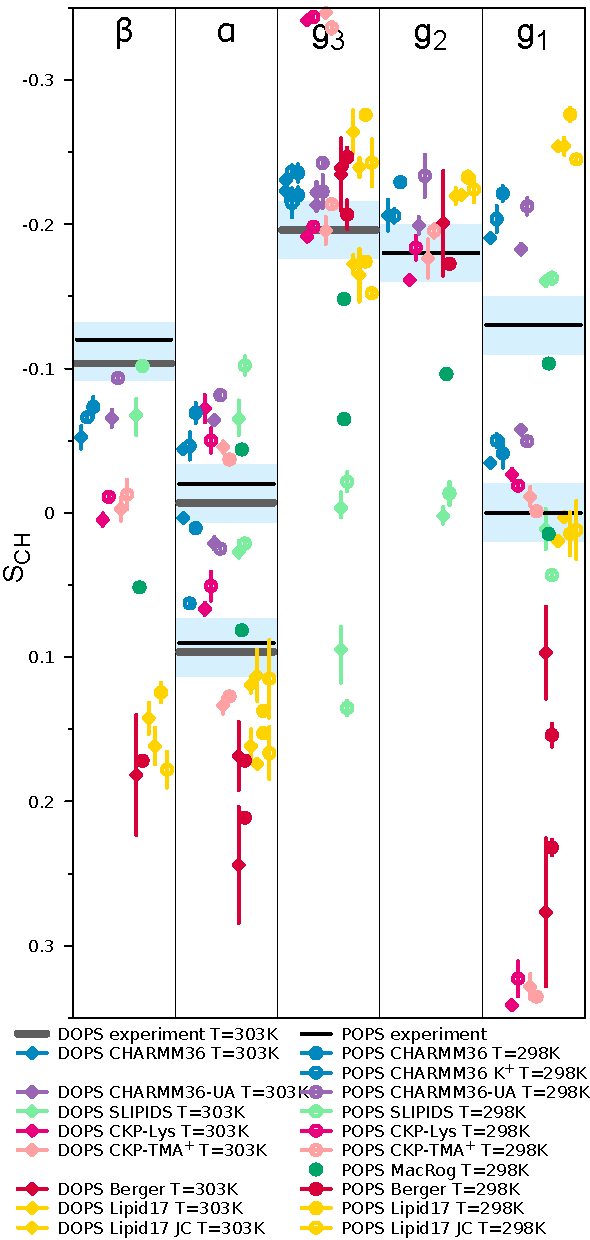
\includegraphics[width=9.0cm]{../Figs/HGorderparametersPS.pdf}
  \caption{\label{HGorderParametersPS}
    Order parameters of PS headgroup ($\beta$ and $\alpha$) and
    glycerol backbone (g$_3$, g$_2$, g$_1$) from NMR experiments (horizontal lines),
    and MD simulations with different force fields (symbols).
    Experimental data for DOPS are measured with 0.1~M of NaCl~\cite{browning80},
    while all the other data are without additional salt.
    The data for DOPS is at 303~K and the data for POPS is at 298~K.
    Light blue areas span 0.04 units around the average of the extremal experimental values,
    in accordance with the expected quantitative accuracy of experiments~\cite{ollila16}.
    The vertical bars shown for all simulation values (excl. MacRog~K$^+$)
    are not error bars, but demonstrate that for these systems
    we had at least two data sets; the ends of the bars mark the extreme values
    from the sets, and the symbol marks their measurement-time-weighted average.
  }
\end{figure}

\begin{figure}[]
  \centering
  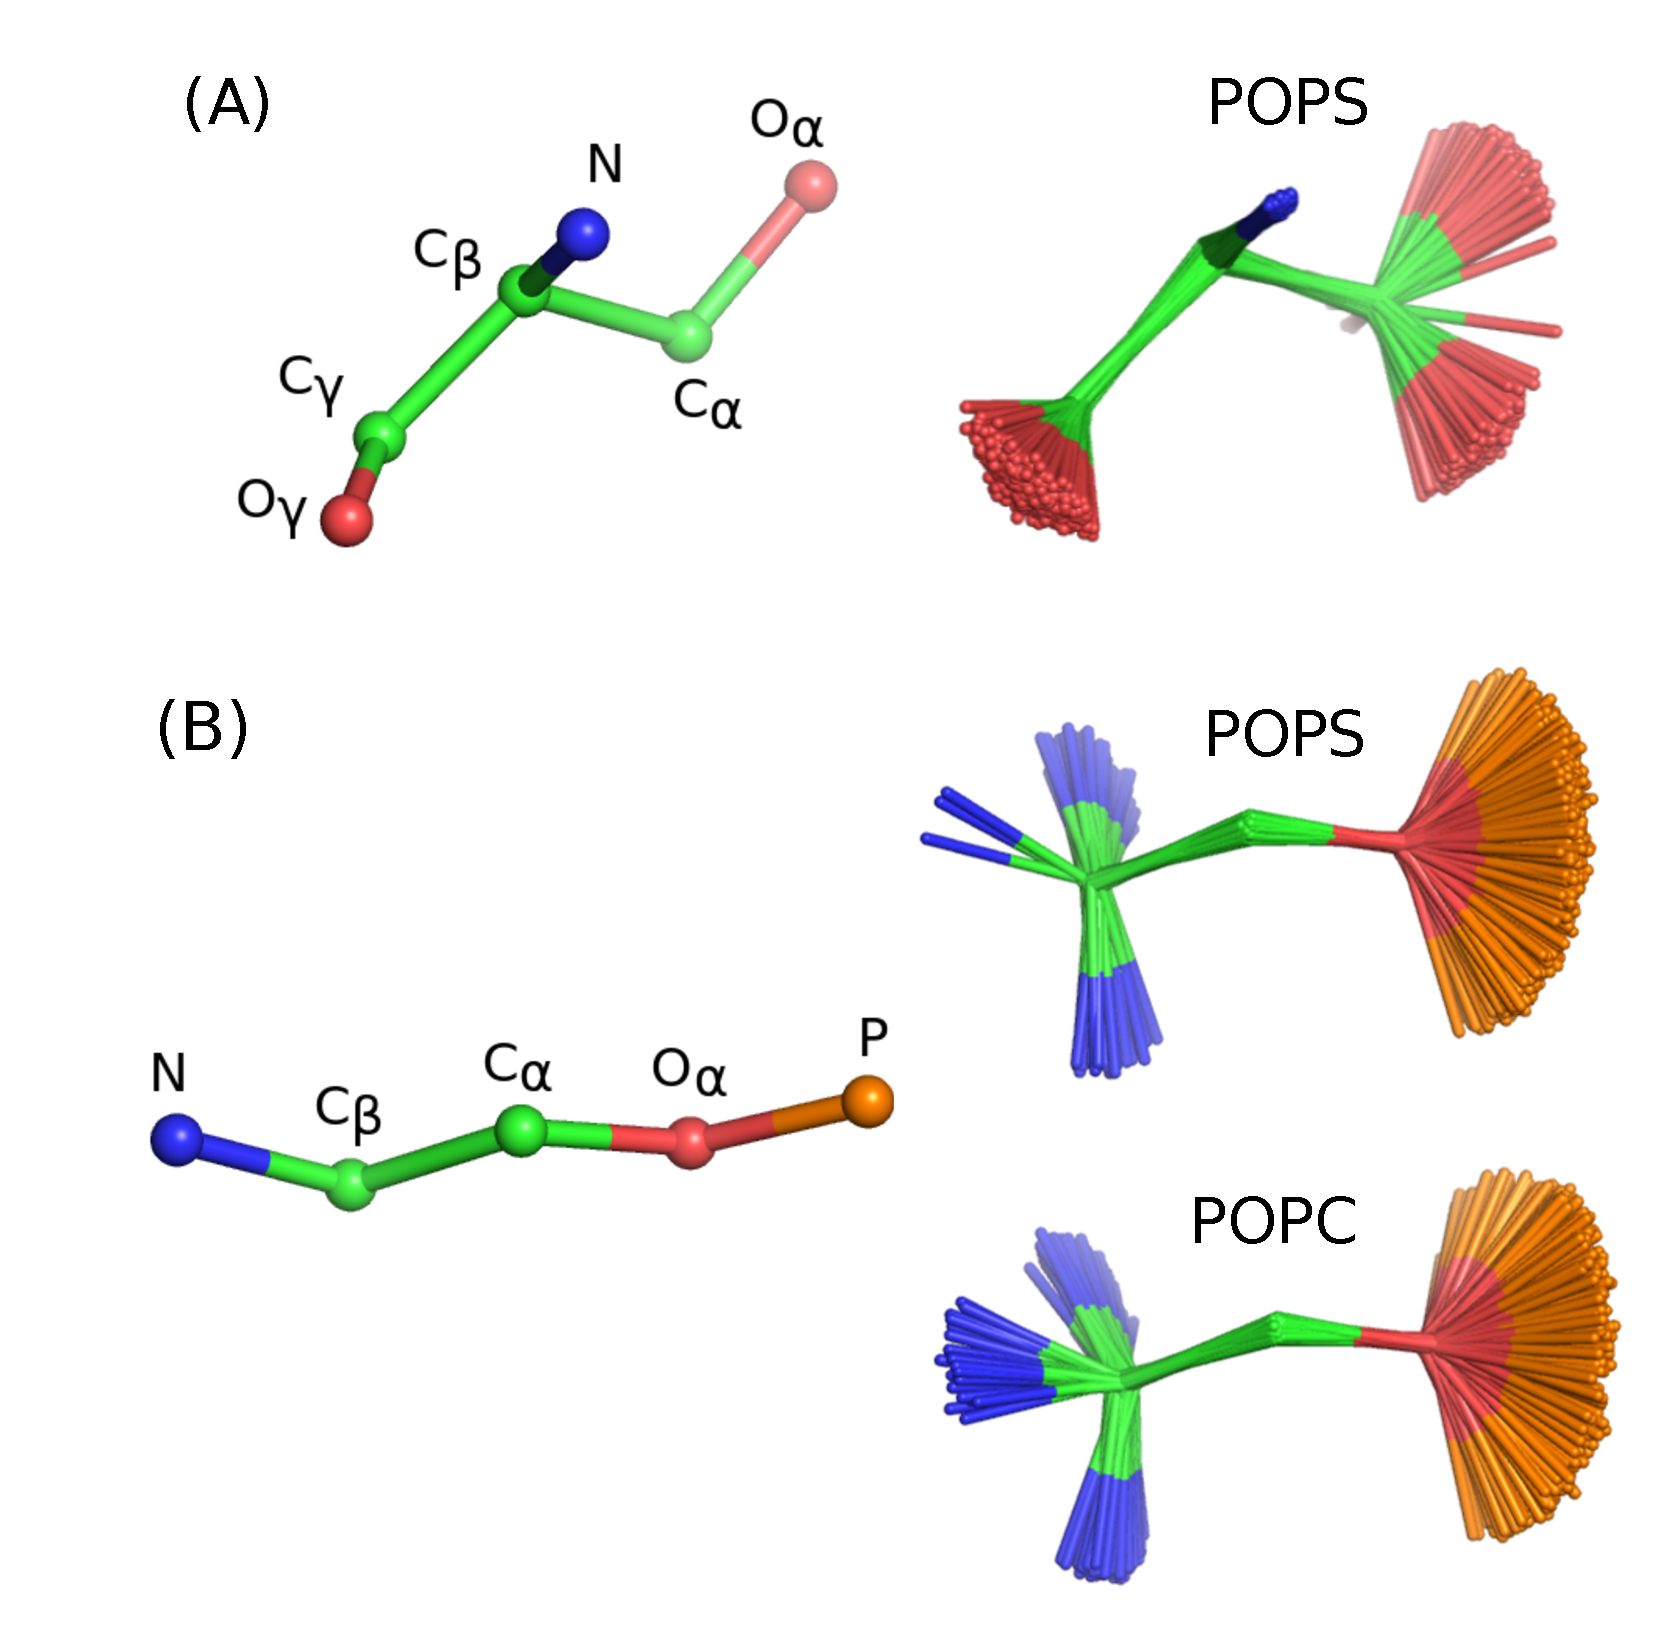
\includegraphics[width=9.0cm]{../Figs/structures.eps}
  \caption{\label{HGstructuresPSandPC}
    Overlayed snapshots from simulations conducted with CHARMM36---the force field producing the best agreement with experiments---demonstrate the conformational fluctuations around
    (A) C$_\alpha$-C$_\beta$-C$_\gamma$-O$_\gamma$ and  O$_\alpha$-C$_\alpha$-C$_\beta$-N
    of PS headgroup and (B) N-C$_\beta$-C$_\alpha$-O$_\alpha$ and C$_\beta$-C$_\alpha$-O$_\alpha$-P
    dihedrals of PS and PC headgroups. The trajectory used for CHARMM36 POPC is available at~\citenum{POPCcharmm36T303K}.
  }

\end{figure}

\begin{figure}[]
  \centering
  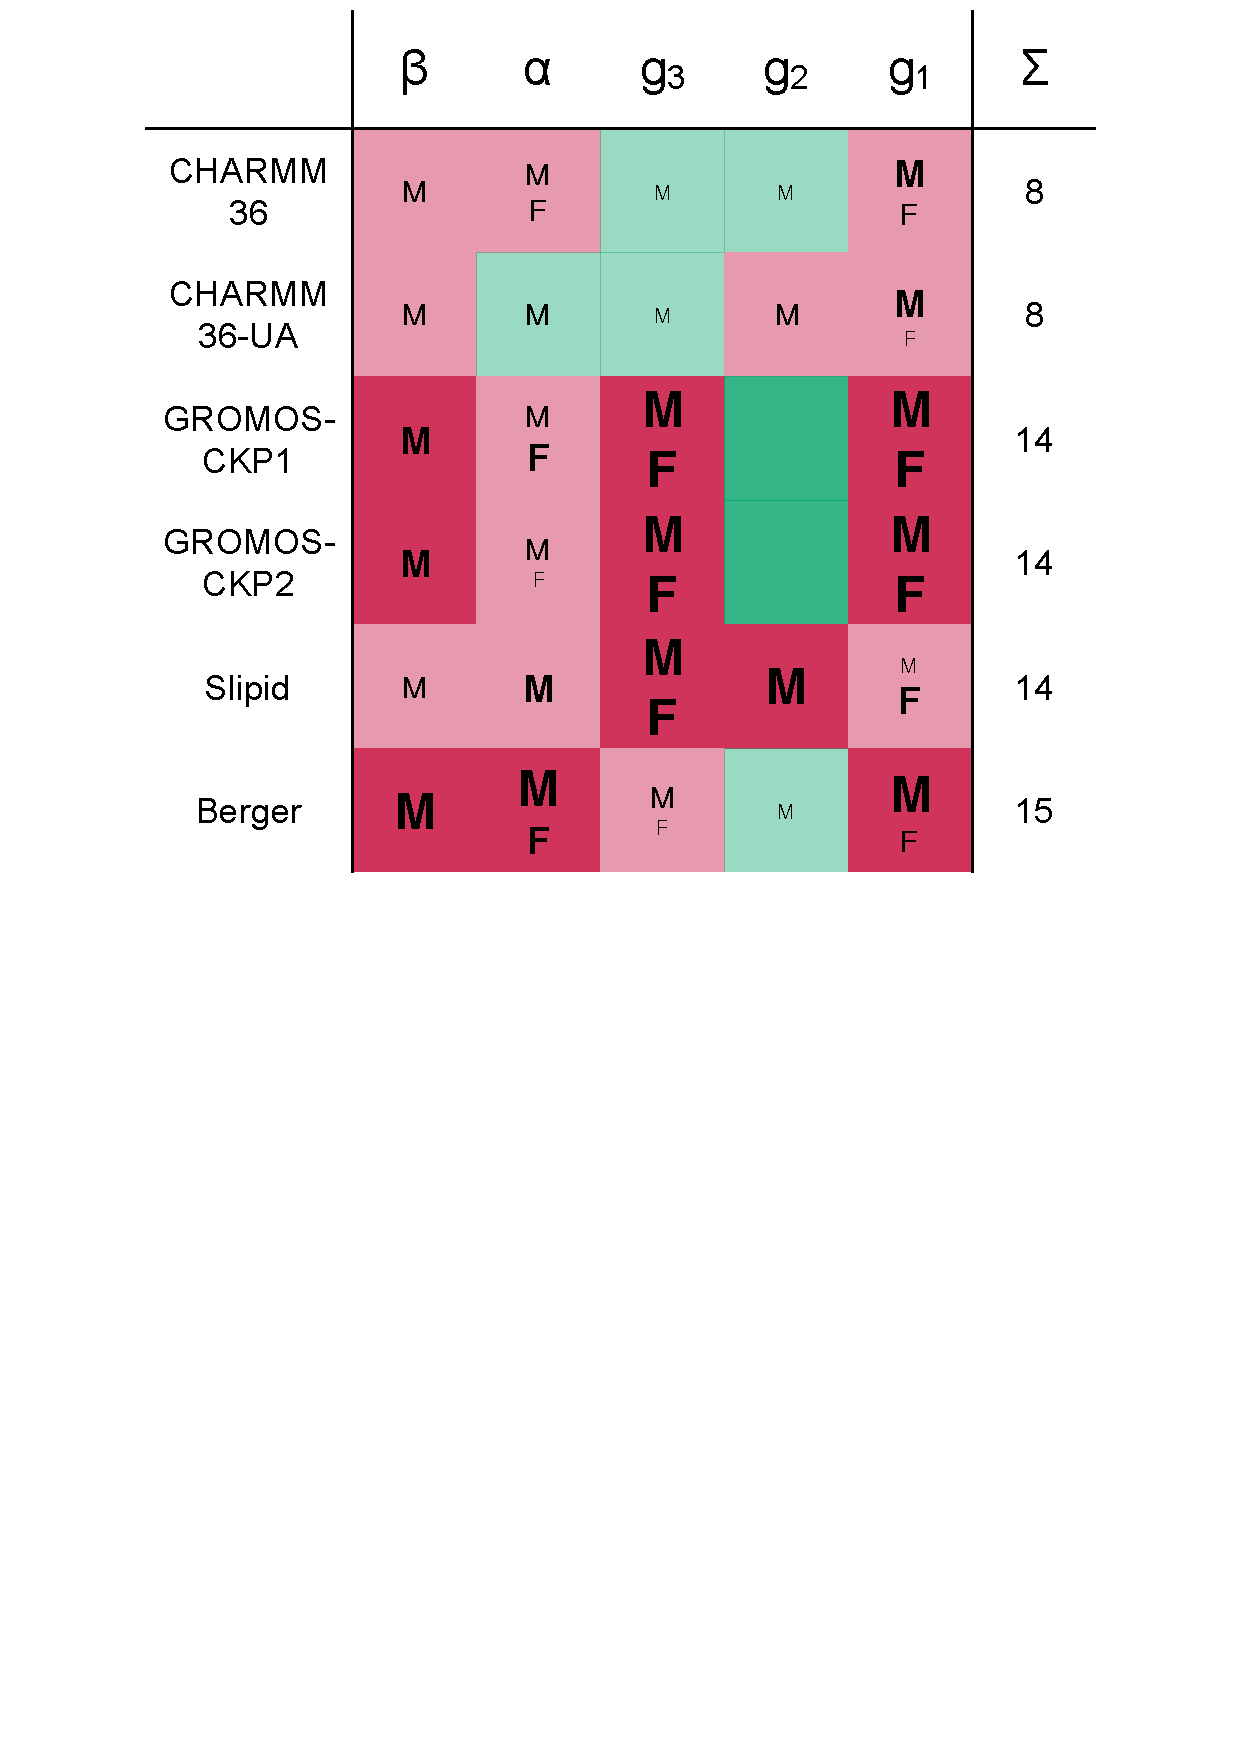
\includegraphics[width=9.0cm]{../Figs/comparisonTablePS.pdf}
  \caption{\label{comparisonTablePS}
    Rough subjective ranking of force fields based on Figure~\ref{HGorderParametersPS}.
    Here {\textsf{\small M}} indicates a magnitude problem, {\textsf{\small F}} a forking problem; letter size increases with problem severity. Color scheme: "within experimental error" (dark green), "almost within experimental error" (light green), "clear deviation from experiments" (light red), and "major deviation from experiments" (dark red). The $\Sigma$-column shows the total deviation of the force field, when individual carbons are given weights of 0 (matches experiment), 1, 2, and 4 (major deviation). For full details of the assessment, see Supplementary Information.
  }
\end{figure}

The different PS MD models produce highly varied  headgroup and glycerol backbone order parameters (Fig.~\ref{HGorderParametersPS})
and structures (Fig.~\ref{HGandGLYstructuresPS} and section~\ref{Diheds} in the SI ),
as previously observed also for PC lipids \cite{botan15}, and none of the models produces a set of order parameters in full agreement with the experiments.
The models perform generally less well for PS than for PC
(Figs.~\ref{HGorderParametersPS} and \ref{comparisonTablePS} vs. Figs. 2 and 4 in Ref.~\cite{botan15}).
which complicates the interpretation of structural differences between PC and PS headgroups. However, concentrating on the headgroup, we see that the best performing models (Slipids, CHARMM36 and CHARMM36ua) do replicate the larger-than-in-PC
forking of the $\alpha$-carbon observed in the experiments and that the Slipids force field additionally correctly produces the significantly
smaller $\beta$-carbon order parameter for PS compared to PC (Fig. \ref{HGorderParametersPS} vs. Fig. 2 in Ref.~\citenum{botan15})
also observed in the experiments (Fig. \ref{HGorderParameters}).

\begin{figure}[!htb]
  \centering
  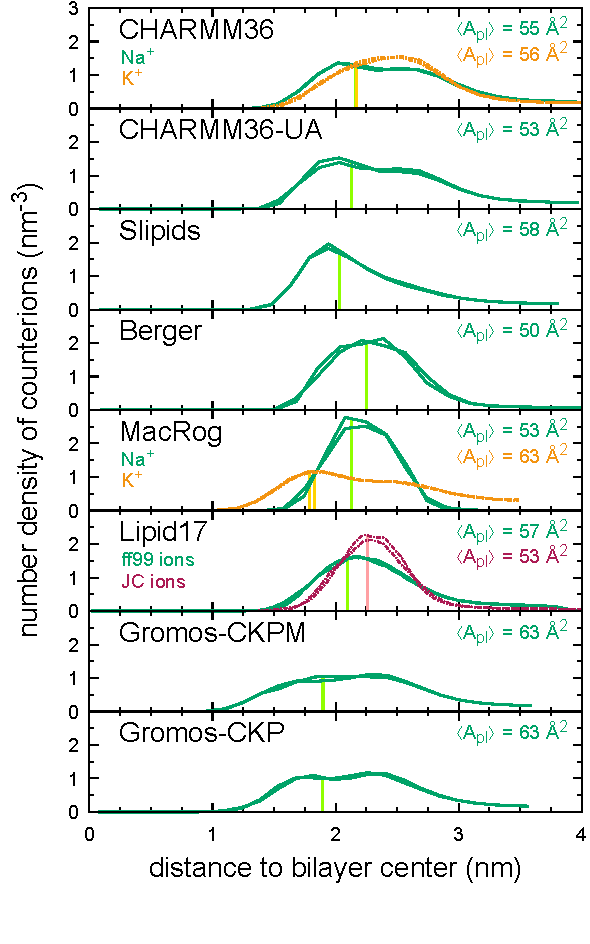
\includegraphics[width=9.0cm]{../Figs/NAdensPOPSformatted.pdf}
  \caption{\label{NAdensPOPS}
    Counterion density profiles along the membrane normal and areas per lipid (A$_{\rm pl}$)
    of POPS lipid bilayer from simulations with different force fields.
    The experimental area per lipid is~62.7~$\pm$~1.3~\AA$^2$~\cite{pan14}.
  }
  \todo{Commented by M. Javanainen in blog:
    MacRog pure POPS is simulated with Verlet cutoff scheme, Piggot is rerunning with group cutoff scheme. Check if affects results \& update figures when ready} \\
\end{figure}


Interestingly, the three models that best fit the experimental data have a narrower distribution in the C$_\alpha$-C$_\beta$-C$_\gamma$-O$_\gamma$
dihedral angle (single peak around 120$^{\circ}$) in comparison to the other models which yield a distribution between two angles (Fig. \ref{dihedralsHG}).
The restricted motion is also visible in the sampled conformations (Figs.~\ref{HGstructuresPSandPC} (A) and \ref{HGandGLYstructuresPS})
suggesting that the rotation of the carboxyl group is limited in the serine headgroup.
In addition, the N-C$_\beta$-C$_\alpha$-O$_\alpha$ dihedral exhibits a more asymmetric
and narrow angle distribution for PS than for PC headgroup in
CHARMM36 simulations that have the best agreement with experiments
(Figs.~\ref{HGstructuresPSandPC} (B) and \ref{dihedralsHGpc}).
% Also, the sampled conformations of glycerol backbone significantly vary between different simulation models (Figs. \ref{dihedralsGLY}, \ref{HGandGLYstructuresPS}, \ref{dihedralsGLYpc} and \ref{HGandGLYstructuresPSPC}),but further analysis is beyond the scope of this work which focuses on the PS headgroup. There is very little actual information in this statement. The variance was already noted above

These results might reflect the increased rigidity proposed in the early experimental studies \cite{browning80,buldt81}, and the suggested characteristic conformations of the PS headgroup can be useful when interpreting experiments. However, as the none of the tested models fully reproduces the experimental order parameters, more accurate MD force fields are required to confirm the correct conformational ensemble.

\subsection{Counterion binding and interactions between PC and PS headgroups}\label{ciBINDINGsection}



\begin{figure}[!tb]
  \centering
  \includegraphics[width=8.0cm]{../Figs/HGorderparametersPCvsPS.eps}
  \caption{\label{HGorderparametersPCvsPS}
    Changes of POPC headgroup order parameters with increasing amount of POPS in POPC:POPS mixtures at 298~K.
    Experimental values are from Ref. \citenum{scherer87} with the signs measured in Ref.~\citenum{ferreira16}.
    The value from the CHARMM36 simulation with sodium is the average of two independent simulations and
    the error bar is given as the difference between the results divided by two.
  }
  \todo{After we know which force field is used for POPC in Gromos-CKP simulations, we might be able to
    add Gromos-CKP data into this plot.}
\end{figure}

\begin{figure}[!tb]
  \centering
  \includegraphics[width=8.0cm]{../Figs/HGorderparametersPSvsPC.eps}
  \caption{\label{HGorderparametersPSvsPC}
    Modulation of POPS headgroup order parameters with increasing amount of POPC in POPC:POPS mixtures at 298~K.
    Experimental values with the signs are measured for pure POPS system in this work.
    The signs are assumed to be the same for the mixture and the values are from Ref. \citenum{roux90}.
    Because the experimental values of POPS in pure and mixed bilayers come from $^{13}$C NMR (this work) and $^2$H NMR (Ref. \citenum{roux90}), respectively,
    the error bars of 0.02 are used here \cite{botan15,ollila16}.
    The y-axis for the $\alpha$-carbon results of POPS (bottom) is shifted
    with the same value for both order parameters such that the lower order
    parameter value from pure POPS is at zero to correctly illustrate the significant forking.
    The values from CHARMM36 and Gromos simulations are averages of two independent simulations and
    the error bars are given as the difference between the results divided by two.
  }
\end{figure}


Membranes containing PS lipids are always accompanied with counterions that
modulate electrostatic interactions between lipids and other biomolecules. MD simulations have suggested
that counterions reduce the area per lipid of PS bilayers compared to PC
bilayers~\cite{pandit02,mukhopadhyay04,pedersen06} by screening the repulsion between charged lipid headgroups. We explore this by quantifying the counterion density profiles along the membrane normal accompanied by the areas per lipid in Fig.~\ref{NAdensPOPS}.
The force fields studied show significant differences in both binding affinity
and distribution of ions at the interface.
The experimental area per lipid (62.7~$\pm$~1.3~\AA$^2$) \cite{pan14} 
is reproduced only in Gromos-CKP and in the MacRog simulation
with potassium counterions, while other models give considerably smaller values.
However, the counterion binding and the concomitant electrostatic screening of the headgroup
repulsion does not fully explain the low area per molecule values
since the MacRog simulation, which has the strongest sodium binding
(the lowest concentrations in bulk water), gives the same area per molecule
as the CHARMM36ua simulation, which has significantly weaker counterion binding
affinity. On the other hand, MacRog simulations with potassium produce a larger area per molecule (63~\AA$^2$) than
with sodium (53~\AA$^2$) in line with the weaker potassium binding affinity (Fig.~\ref{NAdensPOPS}).
The results are in line with the previous study suggesting that the
low areas per molecule in PS lipid bilayers originate from the combination
of both the counterion binding and intermolecular interactions between lipid headgroups~\cite{petrache04}.

\begin{figure*}[ht]
  \centering
  \includegraphics[width=18cm]{../Figs/CHANGESwithCaClPS.eps}
  \caption{\label{changesWITHCaClPS}
   Variation of POPC (left) and POPS (right) headgroup order parameters from POPC:POPS (5:1) mixture
    as a function CaCl$_2$ concentration from experiments \cite{roux90} and different simulations
    at 298K (except the data for Berger model is from simulation of POPC:POPS (4:1) mixture at 310K \cite{ollila07a,melcrova16}). 
    The order parameter values from systems without calcium are set as the zero point of y-axis,
    except for the $\alpha$-carbon order parameter of POPS (bottom, right) for which both order parameters are shifted
    such that the lower order parameter is zero without additional ions. This is to correctly illustrate
    the forking with different concentrations of calcium.
    Potassium counterions are used in MacRog simulations and sodium counterions in Lipid14/17 simulations.
    In CHARMM36 and Berger simulation with added calcium, the charge is neutralized with calcium and monovalent counterions are not present.
  }
%  \todo{Upcoming simulations with original CHARMM36 have been mentioned in the blog:
%    http://nmrlipids.blogspot.com/2017/12/nmrlipids-iv-current-status-and.html?showComment=1520090718976\#c5569269391707740056.
%  these are not necessary, but could be added here if delivered.} \\
\end{figure*}



The experimentally observed modulation of headgroup order parameters
by increasing salt concentration (the molecular electrometer concept) has been previously used to evaluate the cation binding to zwitterionic PC bilayers in simulations \cite{catte16}.
Studying binding of cations to negatively charged lipid bilayers is less straighforward due to the presence of cationic counterions (the lack of a ion-free reference state) and the analysis is further complicated by the artificial aggregation of counterions
observed in some simulations (section \ref{mixtureTOadditionalCIs} in the SI)
% \todo{Why isn't this a problem with PC}.
% SAMULI: The difference between ion-free state (present in PC) and low amount of monovalent ions is larger than
% between counterion only and low amount of monovalent ions in charged lipids. I believe that therefore we can
% make conclusions from smaller ion concentrations without aggregation in PC lipids, but not in charged lipids.
Therefore, we evaluate here the amount of bound charge not by adding salt
(although this is discussed in the SI section \ref{mixtureTOadditionalCIs}),
but by studying the changes of the headgroup order parameters with increasing amount of
negatively charged lipids (and thus increasing amount of cationic counterions) in the bilayer.

Experimentally, the headgroup order parameters of POPC
increase when negatively charged POPS lipids are incorporated in lipid bilayer
(section \ref{HGorderparametersPCvsPEPSPGchol})~\cite{seelig87,scherer87}.
This is reproduced in the MacRog simulations with potassium counterions (Fig. \ref{HGorderparametersPCvsPS}),
which have the weakest binding affinity to POPS lipid bilayers (Fig.~\ref{NAdensPOPS}).
The CHARMM36 and Berger simulations either exhibit no change or show a decrease
in the POPC headgroup order parameters as the amount of POPS increases (Fig. \ref{HGorderparametersPCvsPS}).
Therein, the stronger counterion binding cancels
the effect of negatively charged headgroups and prevents the experimentally observed
increase of headgroup order parameters with growing amount of PS lipids.
Therefore, we suggest that the relatively weak binding of potassium
in the MacRog simulations (Fig. \ref{NAdensPOPS}) produces the most
realistic surface charge density in membranes containing PS lipids,
while the other tested models overestimate the counterion
binding affinity. The results are in line with the behaviour of headgroup order
parameters as a function of added counterions analyzed in section \ref{mixtureTOadditionalCIs}
in the SI.

The reduced forking of the POPS $\alpha$-carbon (Fig.~\ref{HGorderparametersPSvsPC})
together with other experimental results suggest that the PS headgroup structure becomes less rigid when diluted with
POPC~\cite{browning80,buldt81,roux90,roux91,scherer87}.
Unfortunately, none of the tested models correctly reproduce the modulation of POPS headgroup order
parameters with increasing amount of POPC in POPC:POPS mixtures (Fig. \ref{HGorderparametersPSvsPC})
and more accurate force fields are needed
to correctly describe the PC-PS headgroup interactions in MD simulations.
%Having this conclusion in every paragraph gets a bit repetive

\subsection{Ca$^{2+}$ binding affinity to bilayers with negatively charged PS lipids}
\begin{figure}[tb]
  \centering
  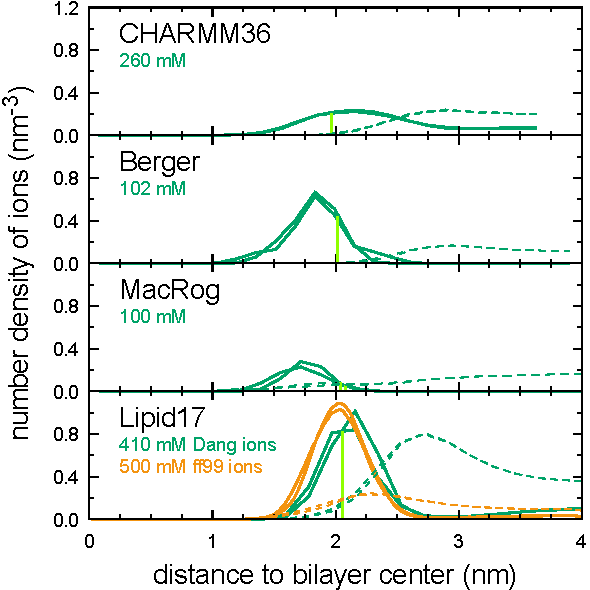
\includegraphics[width=9cm]{../Figs/CAdensPCPSmixtureLOWconsformatted.pdf}
  \caption{\label{CAdensPCPSmixture}
    Number density profiles of Ca$^{2+}$ from POPC:POPS (5:1) mixtures simulated with different force fields.
    The smallest simulated CaCl$_2$ concentrations are shown.
    The density profiles for all the simulated concentrations are given in SI figure \ref{CAdensPCPSmixtureALL}.
  }
  \todo{Should we include also counterions into the plot?} \\
\end{figure}

Calcium binding affinity to membranes containing the negatively charged PS lipids can be
experimentally quantified by measuring the PC lipid headgroup order parameters
from POPC:POPS (5:1) mixtures (section~\ref{electrometerFORmixtures}),
where the measurement is not compromised by the dehydrated lipid-ion complexes and phase separation, and the bilayer remains uniform~\cite{feigenson86,mattai89,roux90,roux91}.
Despite the lack of an ion-free reference state
in the presence of negatively charged lipids, our simulations give
coherent results for POPC headgroup order parameters as a function of
CaCl$_2$ in the POPC:POPS (5:1) mixtures (Fig. \ref{changesWITHCaClPS}).
As expected from the previous study of pure PC lipid
bilayers \cite{catte16}, almost all the tested simulation models overestimate the
experimentally observed~\cite{roux90} decrease of the POPC headgroup order parameters upon increasing Ca$^{2+}$ concentration (Fig. \ref{changesWITHCaClPS}),
indicating too strong calcium binding affinity.
The only exception is the CHARMM36 simulation utilizing the NBfix
interaction for calcium~\cite{kim16}, wherein the modulation of order parameters is underestimated, 
indicating weaker binding affinity than in experiments.
%incorporated in the parameters give by the CHARMM-GUI at the time of running the simulations (January 2018),
Notably, CHARMM36 simulations with the NBfix corrections \cite{venable13,kim16} give similar binding affinities of
calcium and sodium to POPC bilayer (see section \ref{CHARMMcalciumNBfix}), in contrast to the experiments~\cite{cevc90,akutsu81,altenbach84}. This suggests that the calcium binding affinity
is underestimated in CHARMM36 simulations when using the NBfix for calcium \cite{kim16}, but overestimated 
in all the other tested models. This is evident in the calcium density distributions where almost all Ca$^{2+}$ ions bind to the membrane interface in all simulation models except CHARMM36 (Fig. \ref{CAdensPCPSmixture}).


Experimentally, the POPS headgroup order parameters in POPC:POPS (5:1) mixtures
exhibit a strong dependence of CaCl$_2$ with small concentrations that saturates below 100 mM (Fig. \ref{changesWITHCaClPS}).
The $\beta$-carbon order parameter increases with added CaCl$_2$,
whereas the larger $\alpha$-carbon order parameter decreases; a slight increase is observed in
the smaller $\alpha$-carbon value. All these changes are significantly overestimated in the
tested simulation models, including CHARMM36 which underestimated the binding affinity.
Importantly, the different simulation models predict qualitatively different behaviour
for the two POPS $\alpha$-carbon order parameters with added calcium.
For example, both order parameters decrease in Berger, but increase
in MacRog, and in Lipid14/17 and CHARMM36 a more complicated behavior is seen.
This is in contrast to the PC headgroup, where
qualitatively correct reponse to bound ions is observed
in all simulation models, despite significant discrepancies in the headgroup
structures produced in salt-free simulations~\cite{catte16}.
The divergent response of the Berger model may arise from the ring like structures
observed in the headgroup region in this model (Fig. 6 in Ref. \citenum{mukhopadhyay04}).
%These ring like structures are a widespread feature of typical Berger based lipid force
%fields containing explicit hydrogen atoms in the head group
%[REFS https://pubs.acs.org/doi/abs/10.1021/jp900645z and https://www.sciencedirect.com/science/article/pii/S0300908408000692 and https://pubs.acs.org/doi/abs/10.1021/jp9110019]
Therefore, we conclude that
improvement of force fields is necessary to correctly capture the interactions between the
PS headgroup and calcium ions in MD simulations.
\section{Conclusions}

%Lipids with PS headgroups, and their interactions with ions, play an important role in lipid-mediated signaling processes \cite{leventis10,yeung08}. Attemps to use MD simulations to interpret the spectroscopic data have produced contradictory results for the calcium binding details to PSheadgroups \cite{melcrova16,valentine18,hallock18}.  
%Here (as was previously done for PC lipids \cite{botan15,catte16})
Here, we used the headgroup C--H bond order parameters and the open collaboration approach to evaluate the quality
of the headgroup structure and the ion binding affinity 
in available PS MD models.
The main advantage of this approach is the direct connection
between the accurately measurable experimental order parameters and the simulations,
which reduces the ambiguity in the interpretation of experiments.

First, we complemented the available experimental information \cite{browning80,roux90} by measuring the signs of the PS headgroup order parameters,
and then proceeded to compare MD simulation results from several force fields to the experimental data
This revealed that none of the force fields
%tested using the NMRlipids open collaboration
reproduce the PS headgroup order parameters within the experimental accuracy. However,
the best models for the serine headgroup suggested a characteristic rigid conformation for its
carboxyl group. Comparison to the experimentally observed order parameters in POPC:POPS (5:1) bilayers  at varying ion
concentrations \cite{roux90} then showed that the tested MD force fields
overestimate the cation binding affinity to these bilayers with two exceptions: 1) the MacRog simulation with potassium counterions appears to produce the most realistic monovalent ion binding
affinity to PS-containing lipid bilayers, and 2) the CHARMM36 force field with the recently introduced
NBfix correction for calcium \cite{kim16} underestimated the calcium binding affinity.
The experimentally measured response of the PS headgroup order parameter to the bound calcium, and to the dilution of bilayer with zwitterionic PC lipids, were not
qualitatively reproduced in any of the tested force fields, which underlines the need for more accurate
the MD force fields to study the biological functioning of PS lipids.
This is in contrast to the previous results with PC lipids,
where the experimentally measured headgroup order parameter responses to the bound charge
were in qualitative agreement even though the headgroup structures themselves were
incorrect and the cation binding affinities overestimated \cite{catte16}.

We expect our results to pave the way for the development of better MD force fields
for PS lipids. The quality of conformational ensembles produced by the various models can be evaluated based on the headgroup order parameters, which we hope will to guide the development of force fields towards models that correctly reproduce the PS headgroup structures. The cation binding in the force fields can be improved based on the experimental headgroup order parameter data from POPC:POPS (5:1) mixtures under different cation concentrations. This was already demonstrated for POPC using the electronic continuum correction \cite{melcr18}, and a
similar study for POPS is being progressed separately \cite{ECCpops}.


% Tables may be be put in the text as floats.
% Here is an example of the general form of a table:
% Fill in the caption in the braces of the \caption{} command. Put the label
% that you will use with \ref{} command in the braces of the \label{} command.
% Insert the column specifiers (l, r, c, d, etc.) in the empty braces of the
% \begin{tabular}{} command.
%
% \begin{table}
% \caption{\label{} }
% \begin{tabular}{}
% \end{tabular}
% \end{table}

% If you have acknowledgments, this puts in the proper section head.
\begin{acknowledgments}
% Put your acknowledgments here.
  OHSO acknowledges financial support from Academy of Finland (315596),
  Integrated Structural Biology Research Infrastructure of
  Helsinki Institute of Life Science (Instruct-HiLIFE), and
  CSC-IT center for science for computational resources.
  MJ acknowledges financial support from the Emil Aaltonen foundation and
  and CSC-IT center for science for computational resources.
\end{acknowledgments}

\newpage


% Create the reference section using BibTe
\bibliography{refs.bib}

%\newpage
%\section{APPENDIX: The NMR results reported by Tiago Ferreira}

\listoftodos

\end{document}
%
% ****** End of file aiptemplate.tex ******
